% !TeX root = ../main.tex
% Add the above to each chapter to make compiling the PDF easier in some editors.

 \chapter{Approach}\label{chapter:Approach}
 In this chapter we explain the use cases and requirements to design a context-aware pervasive software framework. Then, we illustrate the  proposed architecture and design following from the concepts introduced in the background chapter and taking into account the challenges and possible solutions shown in the foundation chapter. To recap,  our aim is to design a context-aware pervasive software framework to manage and distribute computations while considering resources, dependencies and networking even with no end-to-end path.



\section{Use Cases}
\section{Requirements}
%The framework should
%\begin{itemize}
%	\item  send computations to all or selected nodes.
%	\item  allow computations to carry custom dependencies.
%	\item  allow communication between nodes in a publish-subscribe manner.
%	\item  carry computations forward even without an end-to-end path between sender and receiver.
%	\item  allow computations to receive data as an input or publish data as an output using the communication layer.	
%	\item  send a computations to nodes according to their computation capabilities, available sensors and actuators.
%	\item  send computations to  specific nodes with a given global identifiers.
%	\item  allow computations to be composable locally and globally.
	
%\end{itemize}

%The computations should
%\begin{itemize}
%	\item  be able to access their dependencies.
%	\item  be triggered either by a scheduler or at-will.
%	\item  persist data in any form.
%	\item  access hardware resources such as camera, sensors and actuators.
%	\item  be pervasive and act on their own.
%\end{itemize}

\section{Framework Architecture}
In this section we explain the software framework architecture designed for pervasive environments and challenged networks to distribute and manage computations with their respective resources and dependencies.  The main idea behind this design is to harness the features of node-RED to create, deploy and share computations of any kind. In addition to having SCAMPI as an information-centric, publish-subscribe and delay tolerant messaging system that gives the framework the skill to deliver messages even without an end-to-end path. However, node-RED and SCAMPI are two different environments that cannot manage computations, resources and dependencies on their own. They need a middleware to orchestrate the communication between them.\\


\noindent In general the architecture stack on each node should look like figure \ref{fig:stack}. With SCAMPI at the stack bottom relying only on the JVM. Then on top of SCAMPI is its Java API to communicate with the TCP API of SCAMPI. Afterwards, comes the middleware which acts mediator in between node-RED and SCAMPI. Finally, at the very top exits node-RED to run computations and interact with the user if needed. However, if SCAMPI is used on an android device, there might be no need to run neither the middelware nor node-RED since the device will be  used to transport data from one node to another having no end-to-end path. Below we explain how each component of the system work.
\begin{figure}[H]
	\centering
	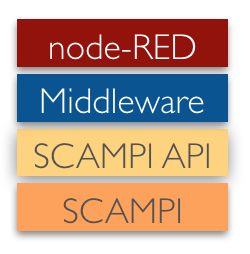
\includegraphics[scale=0.8]{images/stack.png}
	\caption{The framework architecture stack.  }
	\label{fig:stack}
\end{figure}



\subsection{SCAMPI}
As mentioned before SCAMPI is an information-centric, publish-subscribe and delay-tolerant messaging system. In this framework we use SCAMPI to send or receive messages that include computations and data. SCAMPI is also broker-less meaning we do not have to set up a server as broker which is one of the main reasons we chose SCAMPI, in order to be dynamic as possible. The other main reason is to reach nodes which do not have direct connectivity to the publishing node or do not have end-to-end path. \\

\noindent Being a delay-tolerant networking architecture, SCAMPI can use its store-carry-forward routing to deliver messages to challenged environments. In figure \ref{fig:scampi-design}, we show how SCAMPI uses mobile devices to connect nodes that do not have a route or  direct connection and want to exchange messages. In the figure, there are three Raspberry Pi devices running our proposed stack. The first two  have network connection therefore it is rather easy to exchange messages between themselves. However, the third one is isolated, nevertheless it can be connected to a Wi-Fi network or run as an access point. In this case, an android device passing  between network \textit{N1} and \textit{N2} can carry the message bundles from one network and forward it to the other by connecting to both networks alternatingly.  Thus, reaching out to challenged environments that can not be reached using wired or wireless connections.

\begin{figure}[H]
	\centering
	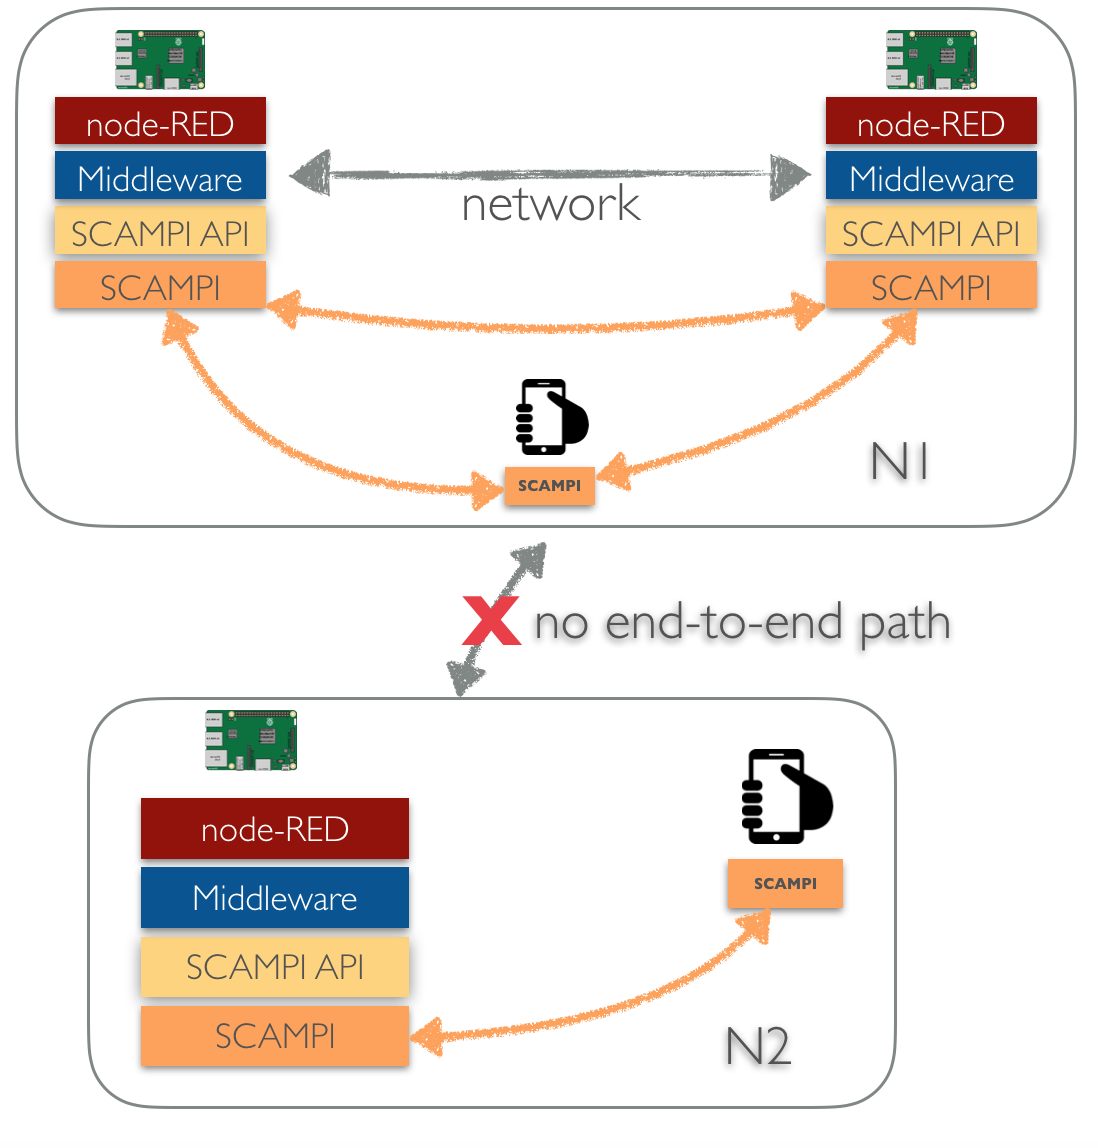
\includegraphics[scale=0.4]{images/scampi.png}
	\caption{SCAMPI synchronization even without an end-to-end path. }
	\label{fig:scampi-design}
\end{figure}

\noindent Being information-centric, data-centric with publish-subscribe pattern and having peer discovery helps us in achieving our dynamic framework without knowing any host names. It  also supports adding and removing nodes at will without any additional configuration. We can also use the general identifiers of the nodes as topics in order to target each of them independently. As stated, SCAMPI does not have any dependencies other than the JVM so we just run it on each node and we are  good to go. \\


\noindent The SCAMPI Java API acts as a client to the server allowing us to publish or subscribe for any topic from the Java environment. Therefore, we are able to extend this API and create a running Java application that uses the TCP API for SCAMPI underneath. The API also allows the client to override the functions for SCAMPI status changes  for instance if it is disconnected, stopped or most importantly when a new message is received. Furthermore, there is a model called \textit{SCAMPIMessage} used to create messages. The model assists in assigning attributes to the message whether strings, integers or even binaries. Also, you can assign meta-data and lifetime to the message.


\subsection{Node-RED}

Node-RED is a tool used for wiring IoT applications, its flows describe the intended computations. It has exporting and importing endpoints for flows via REST which makes it easy to deploy without human interaction.  Flows can be also configured to access certain tables or collections on a running database instance and this configuration can be serialized along with the flow. In this framework whenever a flow wants to send a message to another flow on the same node-RED instance or on other instances, it uses the REST API that the middleware provides to publish and subscribe to data topics. This allows node-RED to send or receive data and allow composability both locally and globally.  Further, node-RED is rich with predefined elements that  can be used to run flows on time intervals, connect to emails, twitter accounts or even access a gpio pin on Raspberry Pi. Node-RED usage is intuitive since it is based on flow-programming, it does not need a developer to create a flow.

\subsection{Middleware}
The middleware is this framework's mediator and the main contribution in this work, it is deployed along with node-RED and SCAMPI on each instance in this architecture. It runs a jar file containing a web application server. It has several duties in orchestrating  SCAMPI messages to node-RED instances.
\begin{itemize}
\item It reads the machine specifications to initialize the machine's resources, sensors and actuators 	.
\item It includes the SCAMPI Java API and has a REST API over it which allows any other script from any other language ("including node-RED") to use the publish subscribe feature of SCAMPI.
\item It analyzes  flows by checking the meta-data  attached to the message thus if the middleware finds out that a flow does not have the necessary hardware requirements, sensors or actuators, it will not deploy the flow. 
\item It is responsible for attaching dependencies of  node-RED flows when one is published, also for putting them into the correct directory when receiving them.
\item It provides a message caching mechanism in order to make sure messages are not handled twice.
\item it provides a mapping between the topics and node-RED flows meaning if one or more flows are interested in the same topic, all of them should get the data.
 \end{itemize}

\subsection{Architecture Usage} \label{subsec:usage}
The following figure \ref{fig:design} explains how the framework works and shows how data flows between the stack components. In this section, we explain the basic usage of the architecture.

\begin{figure}[H]
	\centering
	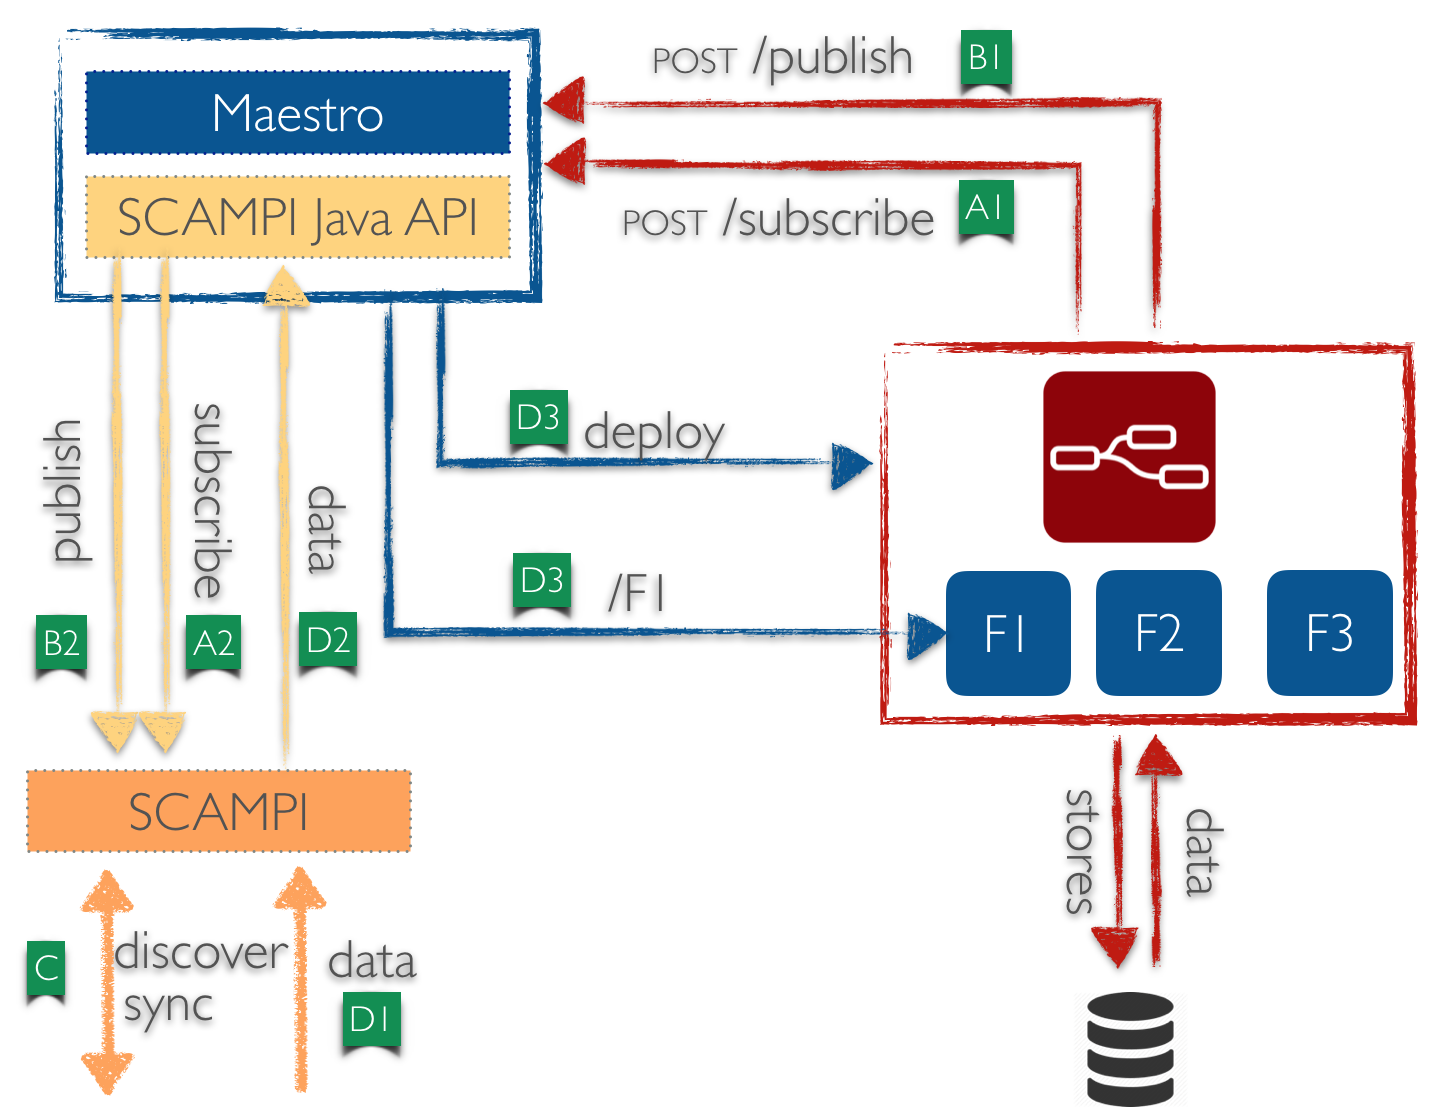
\includegraphics[scale=0.5]{images/design.png}
	\caption{Software framework architecture summary. }
	\label{fig:design}
\end{figure}

\begin{enumerate}[label=(\Alph*)]
 
 \item Flows are developed using node-RED UI, they can include publishing and subscribing REST calls to the middleware. If a flow subscribes to a certain topic, the middelware creates  a topic-endpoint mapping between the topic and an endpoint for this flow specifically. Then send a subscribe request to SCAMPI. If another flow on the same instance wants to subscribe to the same topic, the middleware extends the mapping to include it, hence, once a message is received it gets forwarded to all subscribed flow endpoints. 

 \item When the middleware receives a publish request from node-RED, it attaches the dependencies and an indicator that states if the response should be received by the sending node only. Then the message is forwarded to SCAMPI server.

 \item SCAMPI keeps synchronizing messages and discovering new peers continuously as long as its running. Also, storing some message for the store-carry-forward routing functionality.

 \item When a SCAMPI instance receives data it is forwarded to the middleware, which then checks the meta-data, resources, dependencies and then send the data to the subscribing flows from the topic-endpoint mapping. However, if the message is sent on the computation reserved topic, the middleware will deploy the flow to node-RED.

\end{enumerate}

\section{Summary}

